To generate the `true data' which we will attempt to reconstruct, for $x\in[-L_{x},L_{x}]$, we use the initial conditions 
\begin{align*}
	\eta_{0}(x) = & \frac{1}{E}\sum_{m=-K+1,\neq0}^{K-1} e^{-\left(k_{m}-k_{d}\right)^{2}/2\tilde{\sigma}^{2}}e^{i(k_{m}x+\theta^{(\eta)}_{m})}\\
	q_{0}(x) = & \frac{1}{E}\sum_{m=-K+1,\neq0}^{K-1} e^{-\left(k_{m}-k_{d}\right)^{2}/2\tilde{\sigma}^{2}}e^{i(k_{m}x+\theta^{(q)}_{m})}\\
\end{align*}
where $\theta^{(\eta,q)}_{-m} = -\theta^{(\eta,q)}_{m}$, $k_{m}=\pi m/L_{x}$, and $E$ is the $l_{2}$ normalization condition
\[
E = \left(\sum_{m=-K+1,\neq0}^{K-1} e^{-\left(k_{m}-k_{d}\right)^{2}/\tilde{\sigma}^{2}}\right)^{1/2}.
\]
The phases $\theta^{(\eta,q)}_{m}$ are randomly chosen from a uniform distribution over the interval $[0,2\pi]$, and the $\neq0$ means that both the initial surface and velocity potential have zero spatial mean. Throughout the remainder of this section we choose the primary direction of propagation, $k_{d}$, so that $k_{d} = \pi/L_{x}$.  Thus, in the limit as $\tilde{\sigma}\rightarrow 0$, we go to the monochromatic initial conditions
\[
\eta_{0}(x) \sim \cos\left(\frac{\pi}{L_{x}}x +\theta^{(\eta)}\right), ~ q_{0}(x) \sim \cos\left(\frac{\pi}{L_{x}}x +\theta^{(q)}\right), ~ \tilde{\sigma} \sim 0.
\]
Note, our scaling choices ensure that each initial condition is $\mathcal{O}(1)$ in magnitude, which is consistent with the introduction of $\epsilon$ above as a measure of the effective surface-wave amplitude.  To generate the high-order numerics, we use a pseudo-spectral scheme with $K_{T}=2K=256$ modes and a 4th-order Runge--Kutta scheme with an integrating factor and time step $dt=.01$. We take $\epsilon=.1$ and $\mu=\sqrt{\epsilon}$ since this is consistent with the scaling choices made to derive classic nonlinear shallow water models such as the Korteweg--de Vries equation.  The number of terms used in the DNO expansion is $M=14$, which generally ensures machine precision accuracy for relatively long time evolutions.  

As for how we assimilate data, we set the number of ensemble members to be $N_{e}=200$.  To initialize the filter, we use the following initial conditions for $j=1,\cdots,N_{e}$   
\begin{align*}
	\eta^{(j)}_{0}(x) = & \frac{1}{E}\sum_{m=-K+1,\neq0}^{K-1} e^{-\left(k_{m}-k_{d}\right)^{2}/2\tilde{\sigma}^{2}}e^{i(k_{m}x+\theta^{(\eta,j)}_{m})}\\
	q^{(j)}_{0}(x) = & \frac{1}{E}\sum_{m=-K+1,\neq0}^{K-1} e^{-\left(k_{m}-k_{d}\right)^{2}/2\tilde{\sigma}^{2}}e^{i(k_{m}x+\theta^{(q,j)}_{m})}\\
\end{align*}
Note, by building our ensembles in this way, we are tacitly assuming that we know the initial power spectrum of the waves, leaving the only unknown to be the phases of each member of the ensemble.  This assumption is consistent with the use of results from spectral-wave modeling to approximate the behavior of essentially random-sea states.  
Further, per our scaling choices, we have that the time scale $\tau_{s} = L/\sqrt{gH}$ is given by
\[
\tau_{s}=\frac{L}{\sqrt{gH}} = \sqrt{\frac{H}{\epsilon g}} = \sqrt{H/1m}s = 10 s, ~H=100 m.
\]
If we assume a relatively conservative sampling rate of 10 times per second, then we could choose a non-dimensional sampling rate of up to $dt_{s} = .05$, equal above to the time step of the numerical solver.  However, this would not allow us to study the predictive power of our filtering process.  Thus, we choose $dt_{s}=.5$, or a cycle of $5s$ between data assimilation events.  

We likewise use a 4th-order Runge--Kutta scheme with an integrating factor in order to perform the analysis to forecast update.  Each simulation is run up to $t_{f}=20$, or about $200s$, representing a reasonably realistic length of time.  Lastly, we choose the magnitude of the covariance in the error associated with the data to be $\sigma=.1$.  We note this value is an arbitrary choice in the Ensemble Kalman Filter, and should be chosen large enough to maintain invertibility in the computation of the gain matrix.  

\subsection*{Eularian Data Assimilation Results}
In the following figures, we look at comparisons between using two and four points of measurment as well as varying the degree of nonlinearity used in our modelling from $M=0$ terms used in the DNO, corresponding to a stricly linear model, to $M=1$, and then $M=14$.  Note, the error, $\mathcal{E}(t)$, is computed from the relative difference in the $L_{2}$ norm, i.e.    
\[
\mathcal{E}(t) = \frac{\left|\left|\eta_{a}(\cdot,t)-\eta_{tr}(\cdot,t)\right|\right|_{2}}{\left|\left|\eta_{tr}(\cdot,t)\right|\right|_{2}}.
\]

The results seen in Figures \ref{fig:dno_0}, \ref{fig:dno_1}, and \ref{fig:dno_14} are in part as expected.  Generally, four points of measurement is markedly better than two, and as seen in particular by comparing differences in power spectra, for the relatively long times, again $t_{f}=20$, we run the simulations, the addition of nonlinearity to the model through the introduction of higher-order terms in the DNO improve accuracy.  
\begin{figure}[!h]
	\begin{tabular}{c}
		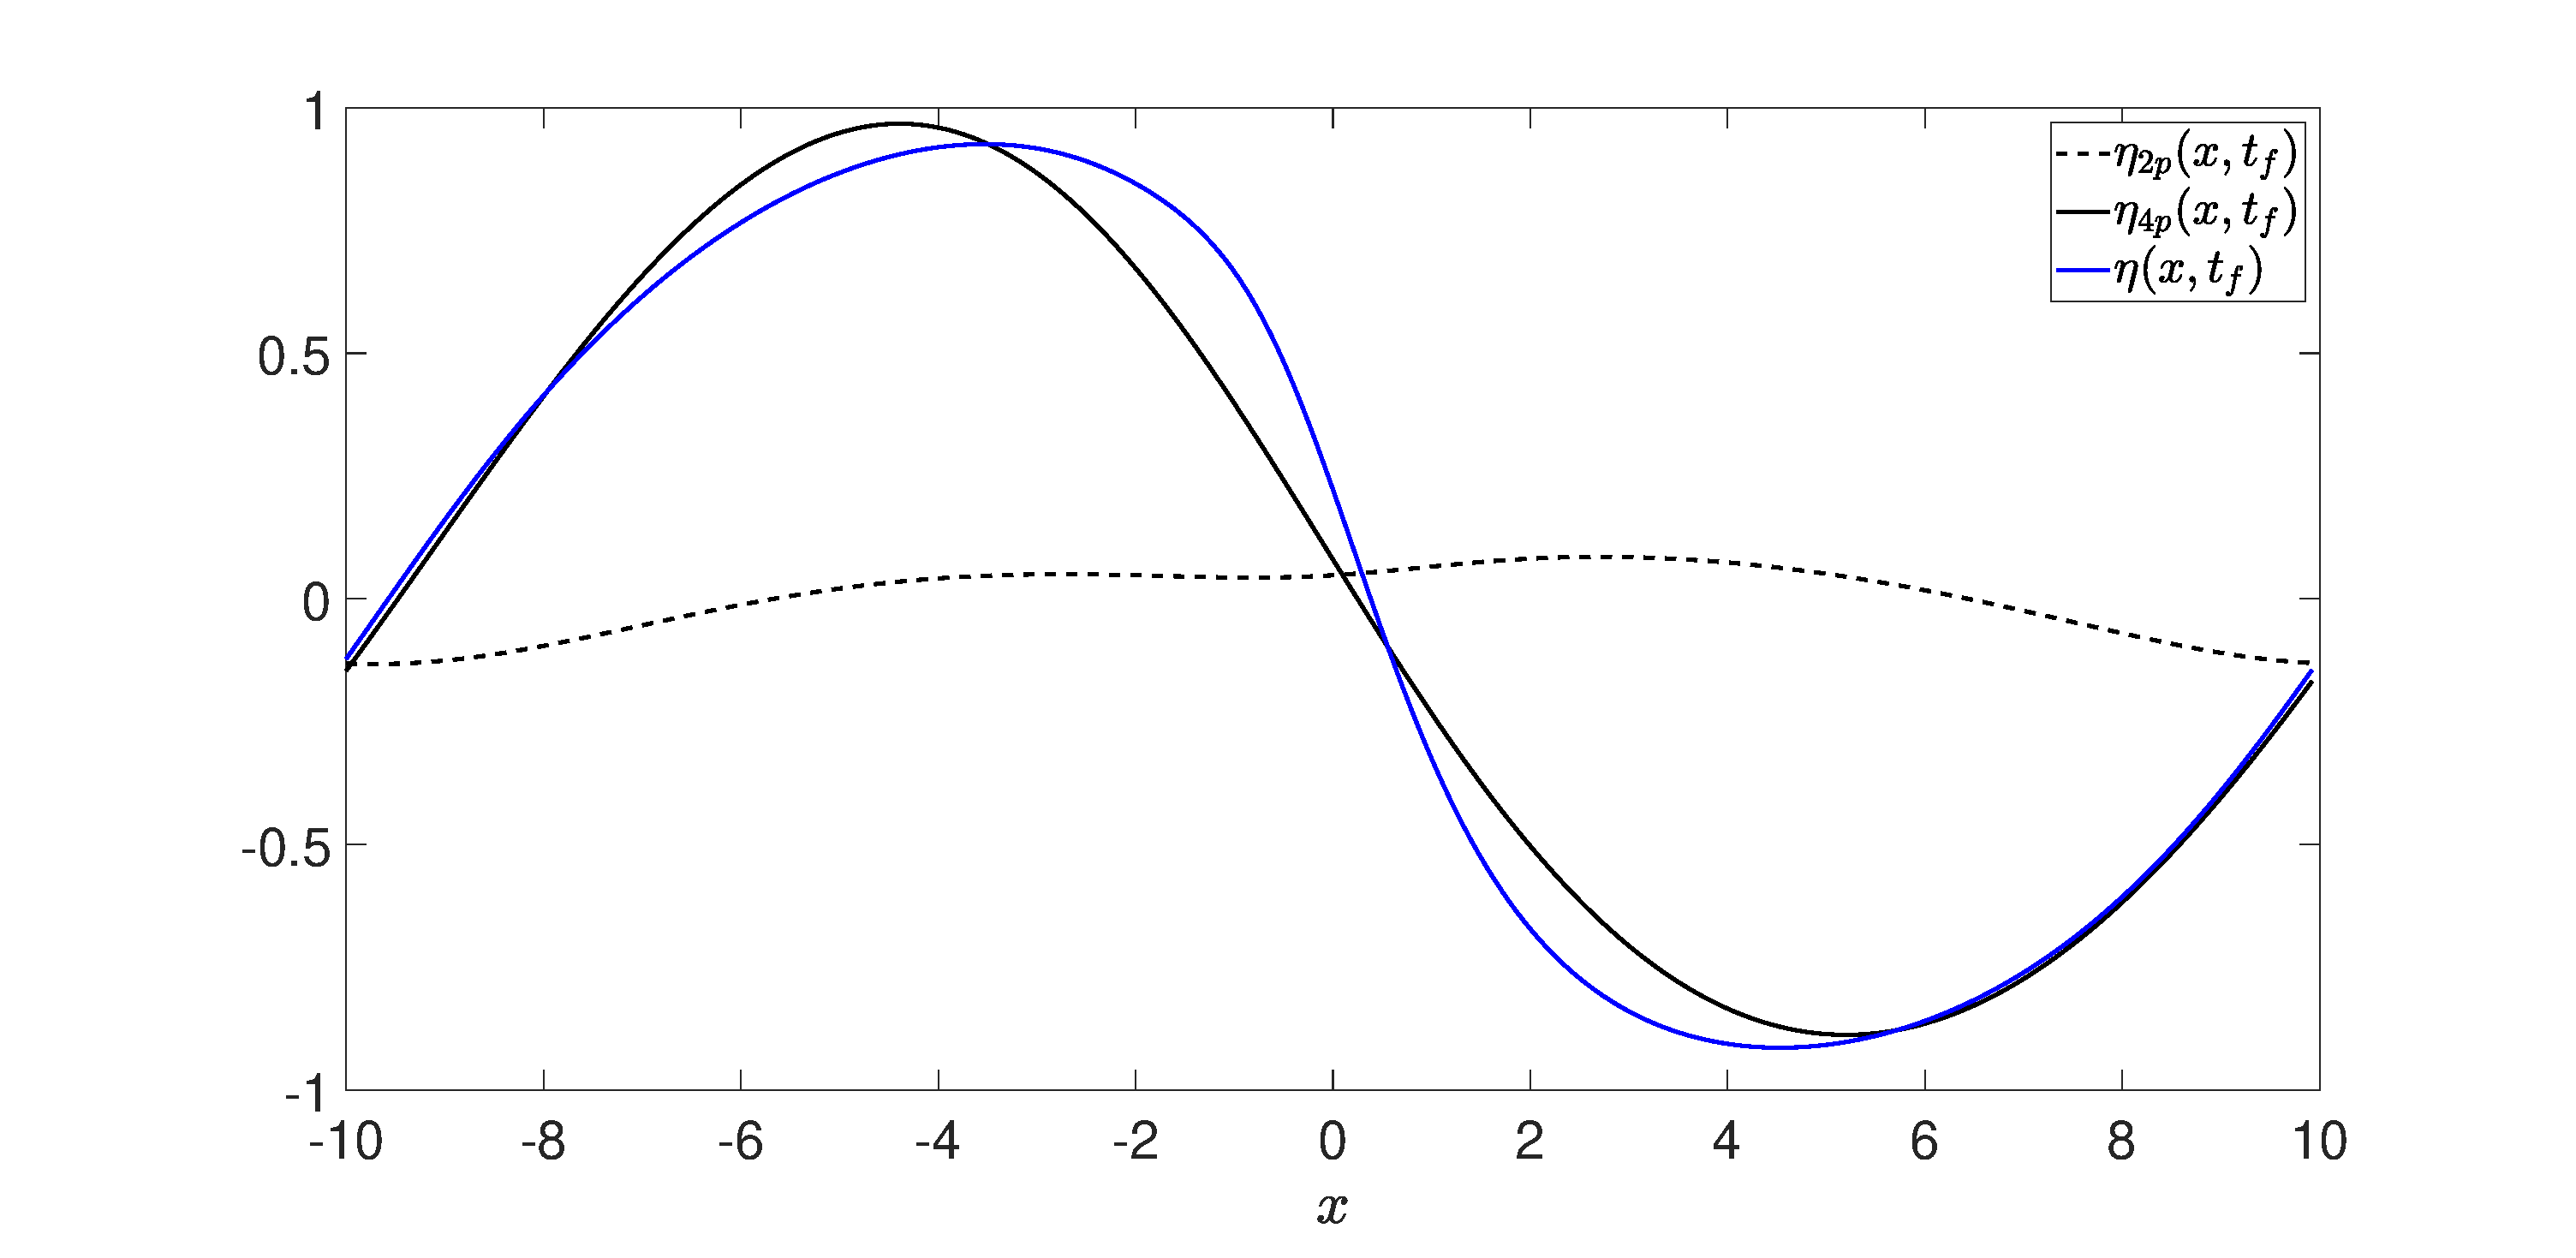
\includegraphics[width=.8\textwidth]{./Images/pwise_sig_pt1_srate_pt5_Nens_200_Np_4_tf_20_M_0}\\
		(a)\\
		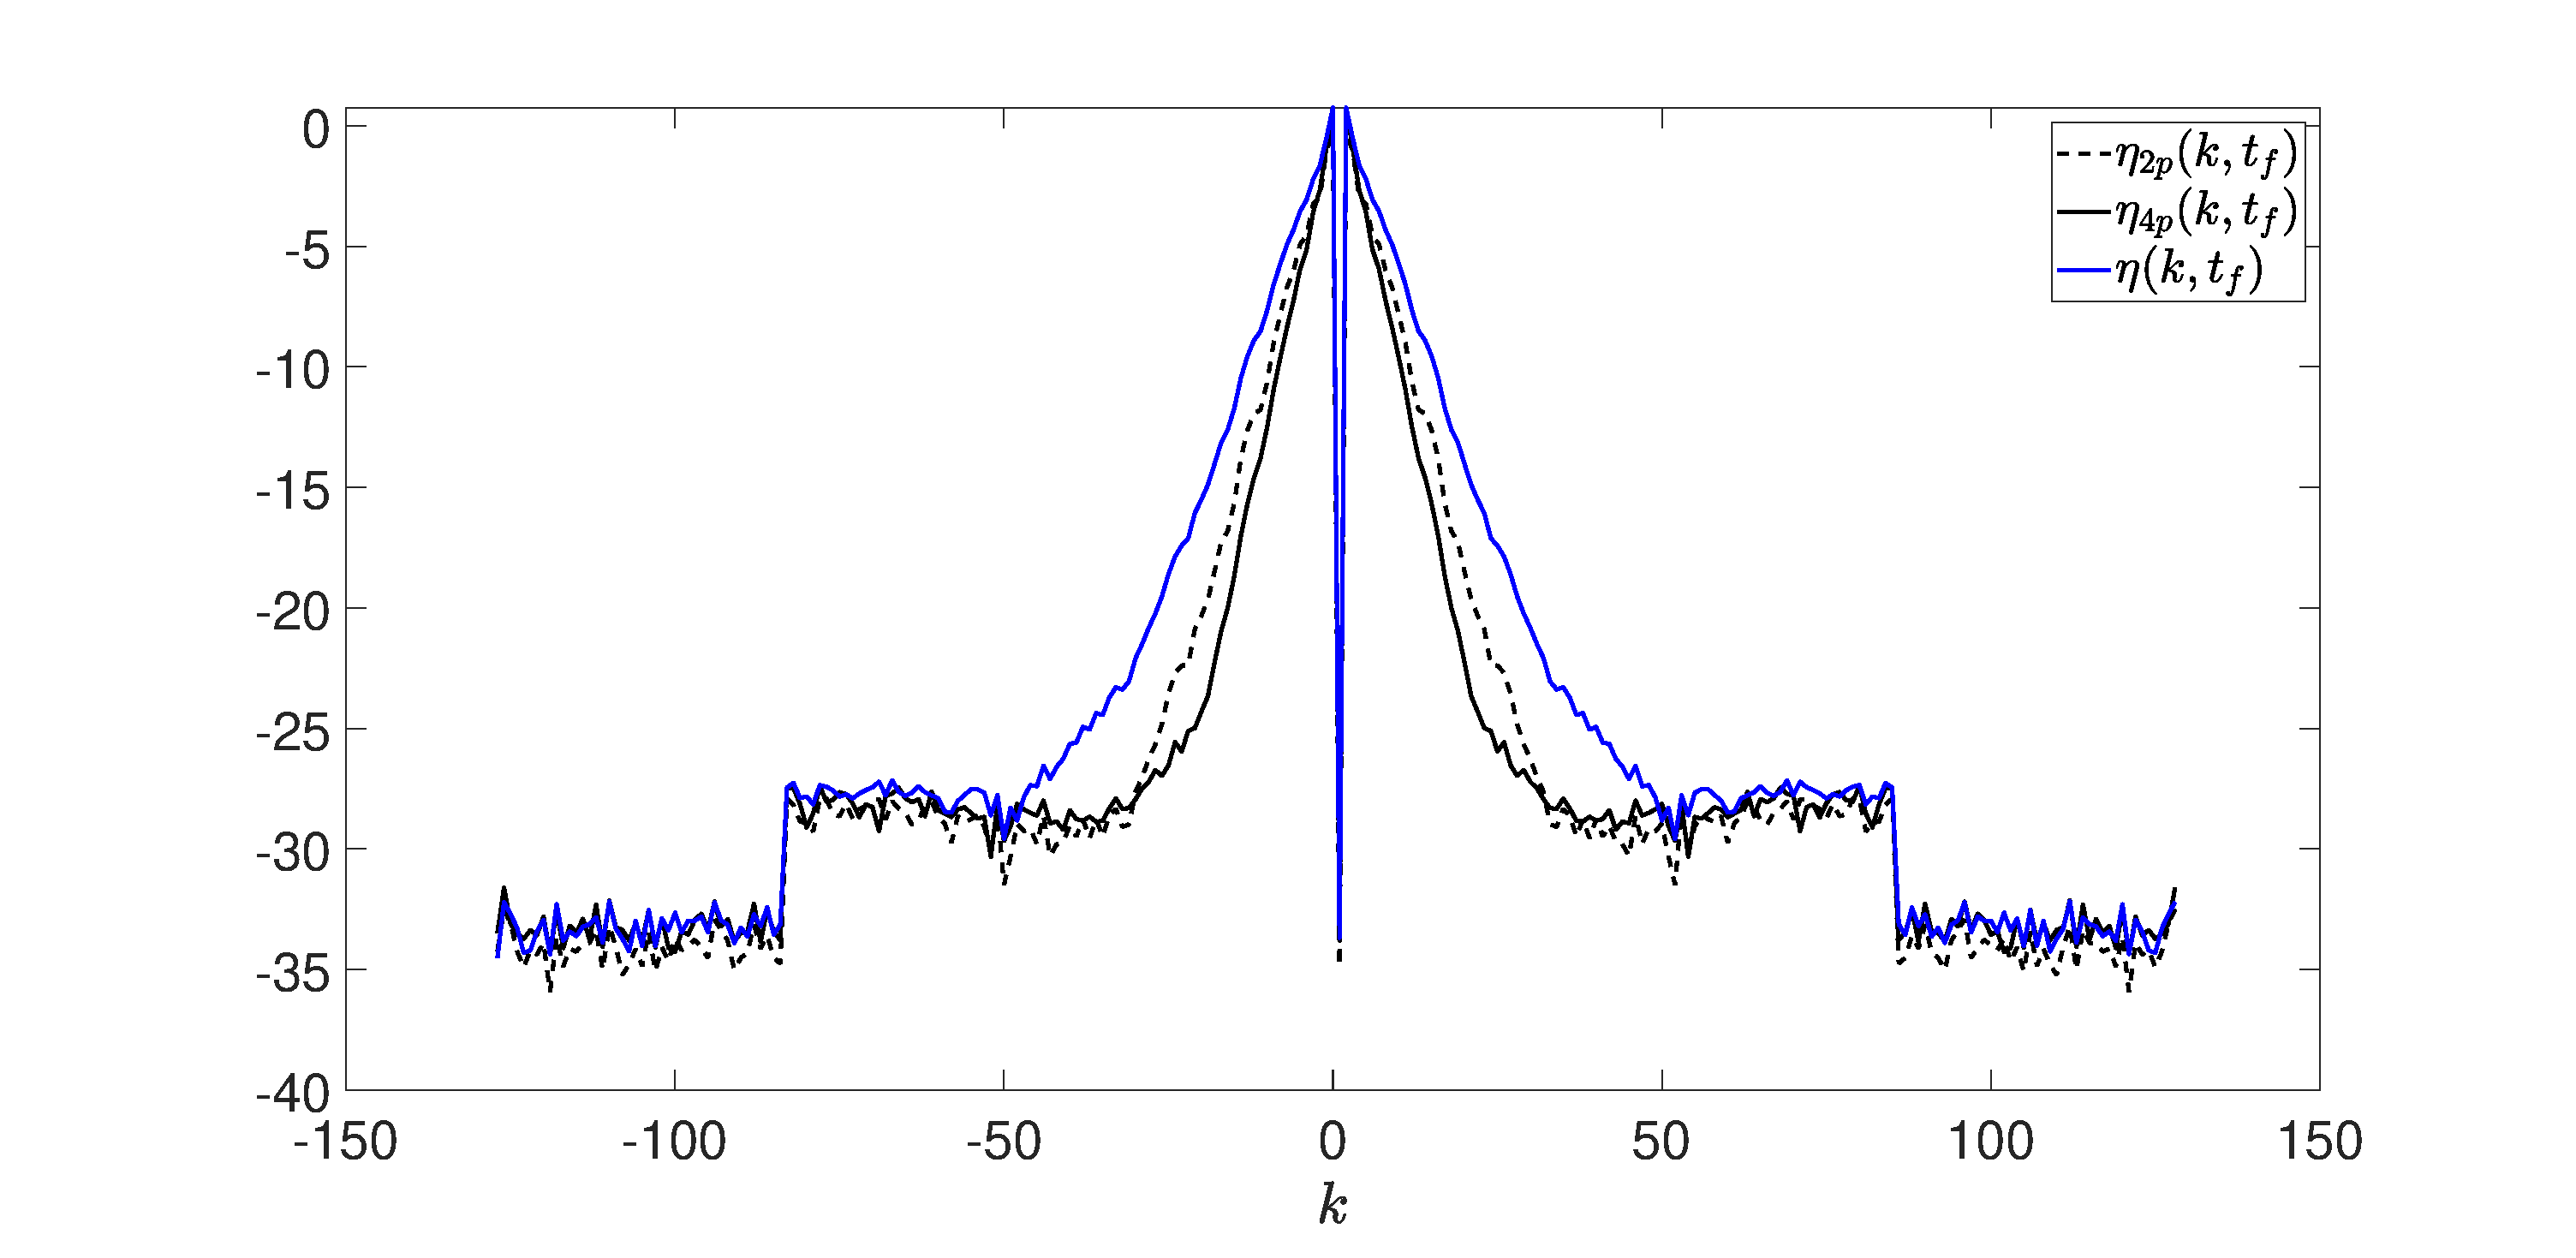
\includegraphics[width=.8\textwidth]{./Images/pspec_sig_pt1_srate_pt5_Nens_200_Np_4_tf_20_M_0}\\
		(b)\\
		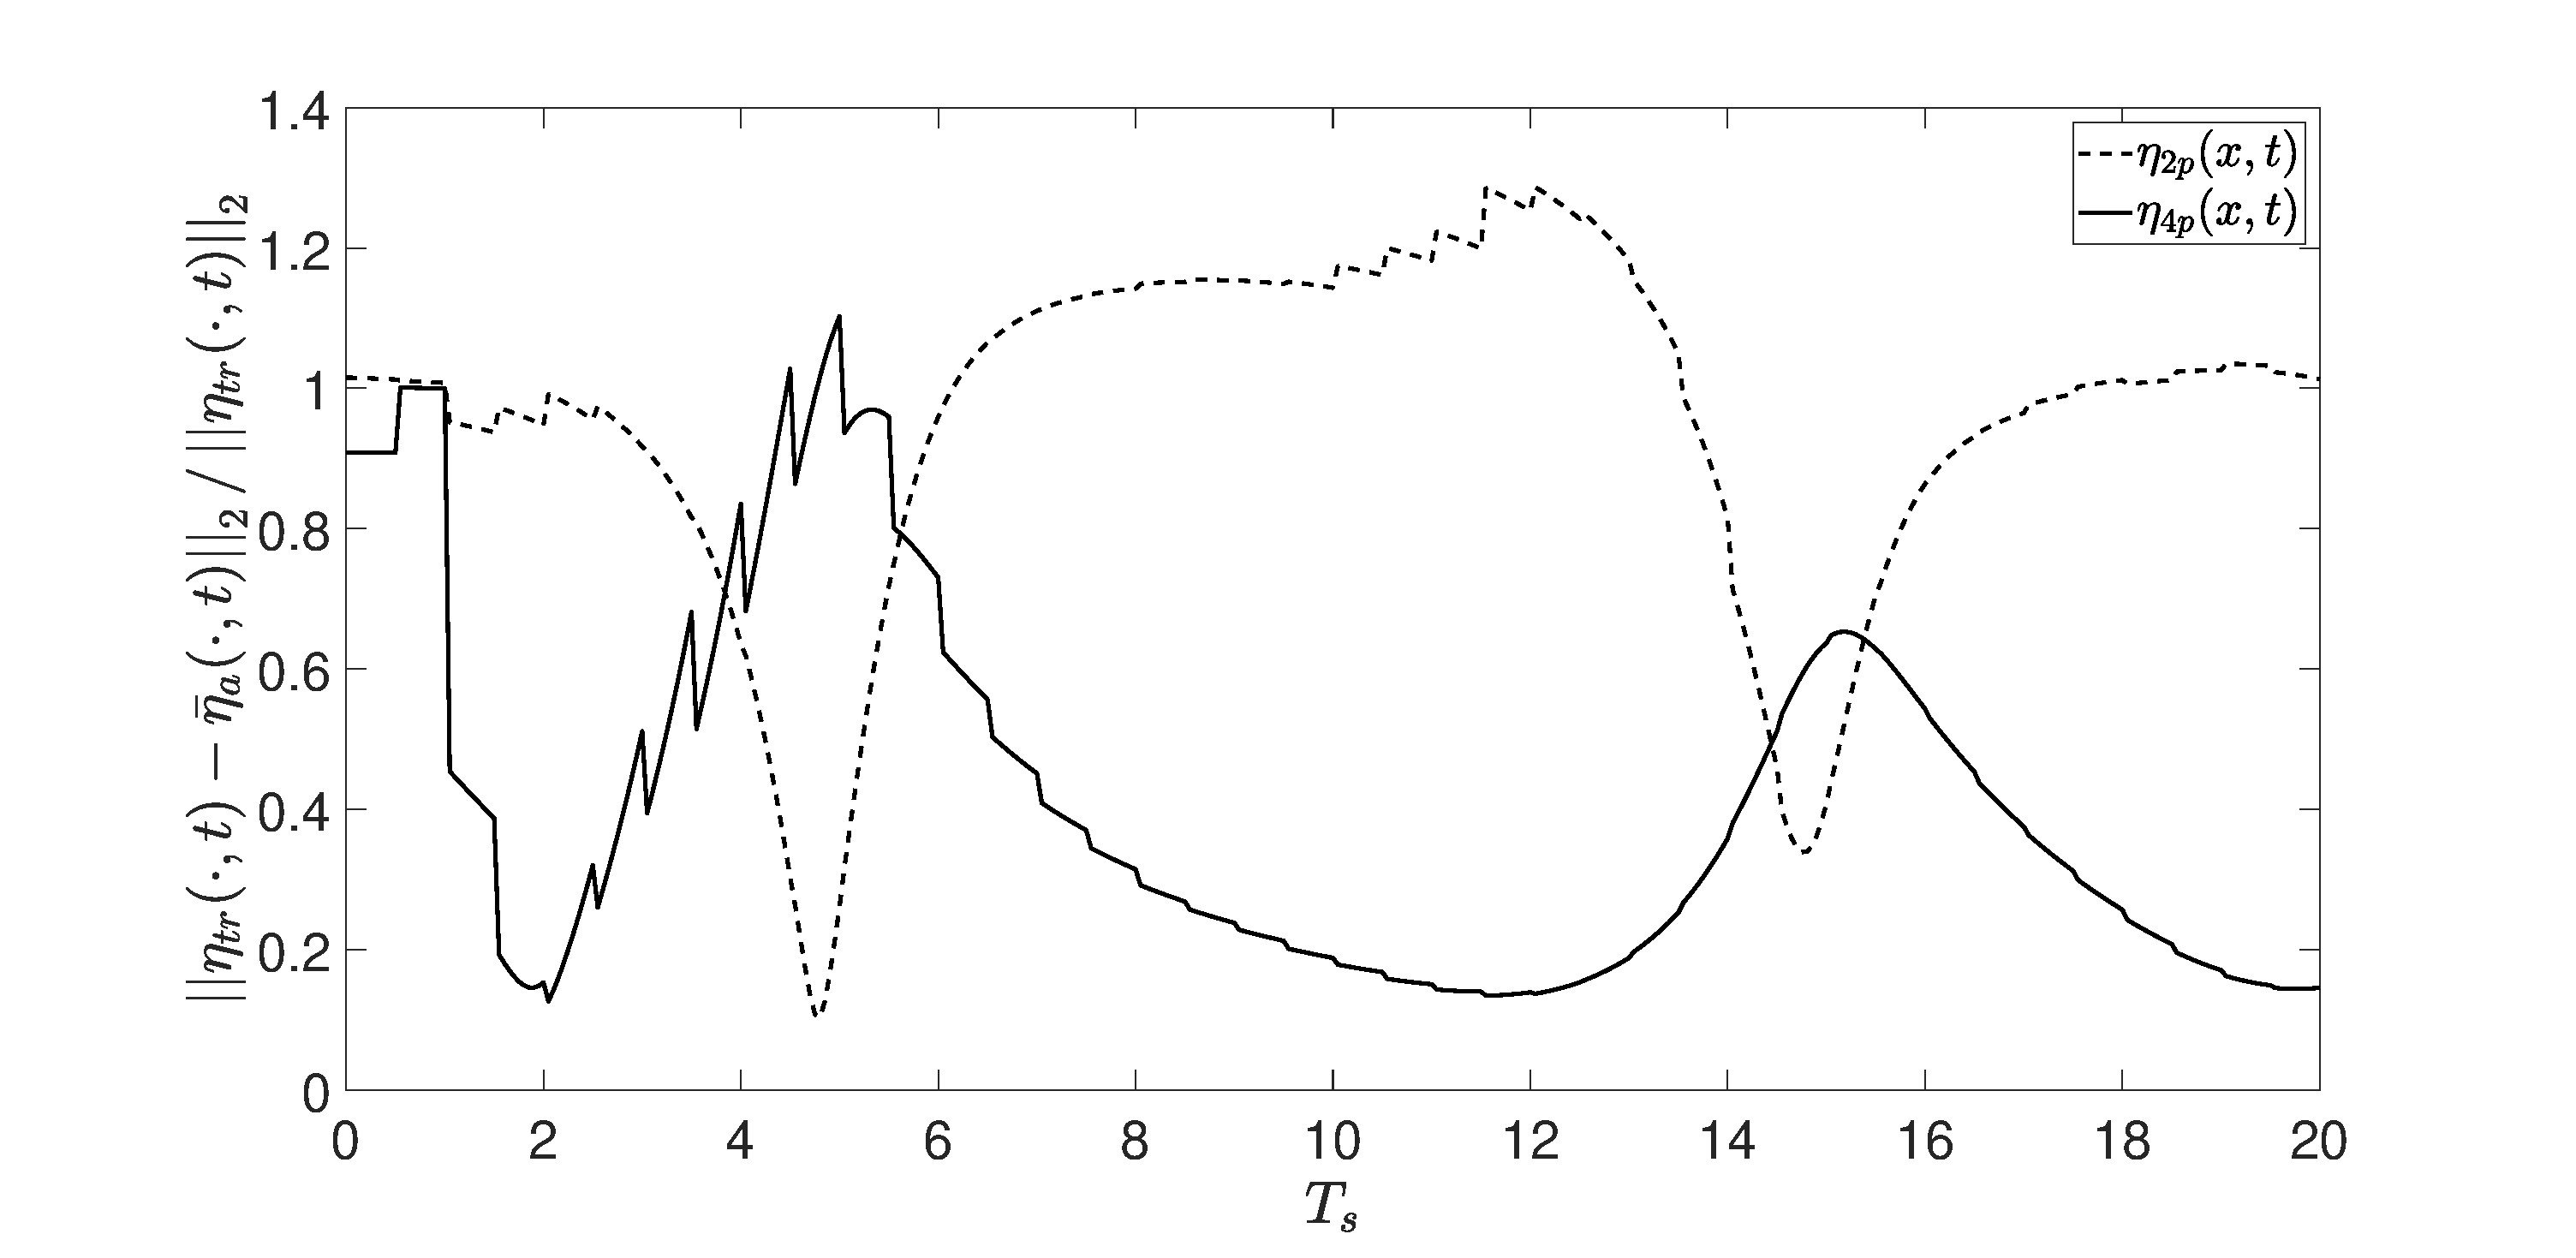
\includegraphics[width=.8\textwidth]{./Images/error_sig_pt1_srate_pt5_Nens_200_Np_4_tf_20_M_0}\\
		(c)	
	\end{tabular}	
	\caption{The pointwise-approximations (a) and power-spectrum approximations (b) at $t_{f}=20$, and error (c) measuring at two (- -) and four points (--) using $M=0$ terms in the DNO.  The data-assimalation rate is $\delta t_{s}=.5$, so that the model is predicting behavior in between assimation events.}
	\label{fig:dno_0}
\end{figure}

\begin{figure}[!h]
	\begin{tabular}{c}
		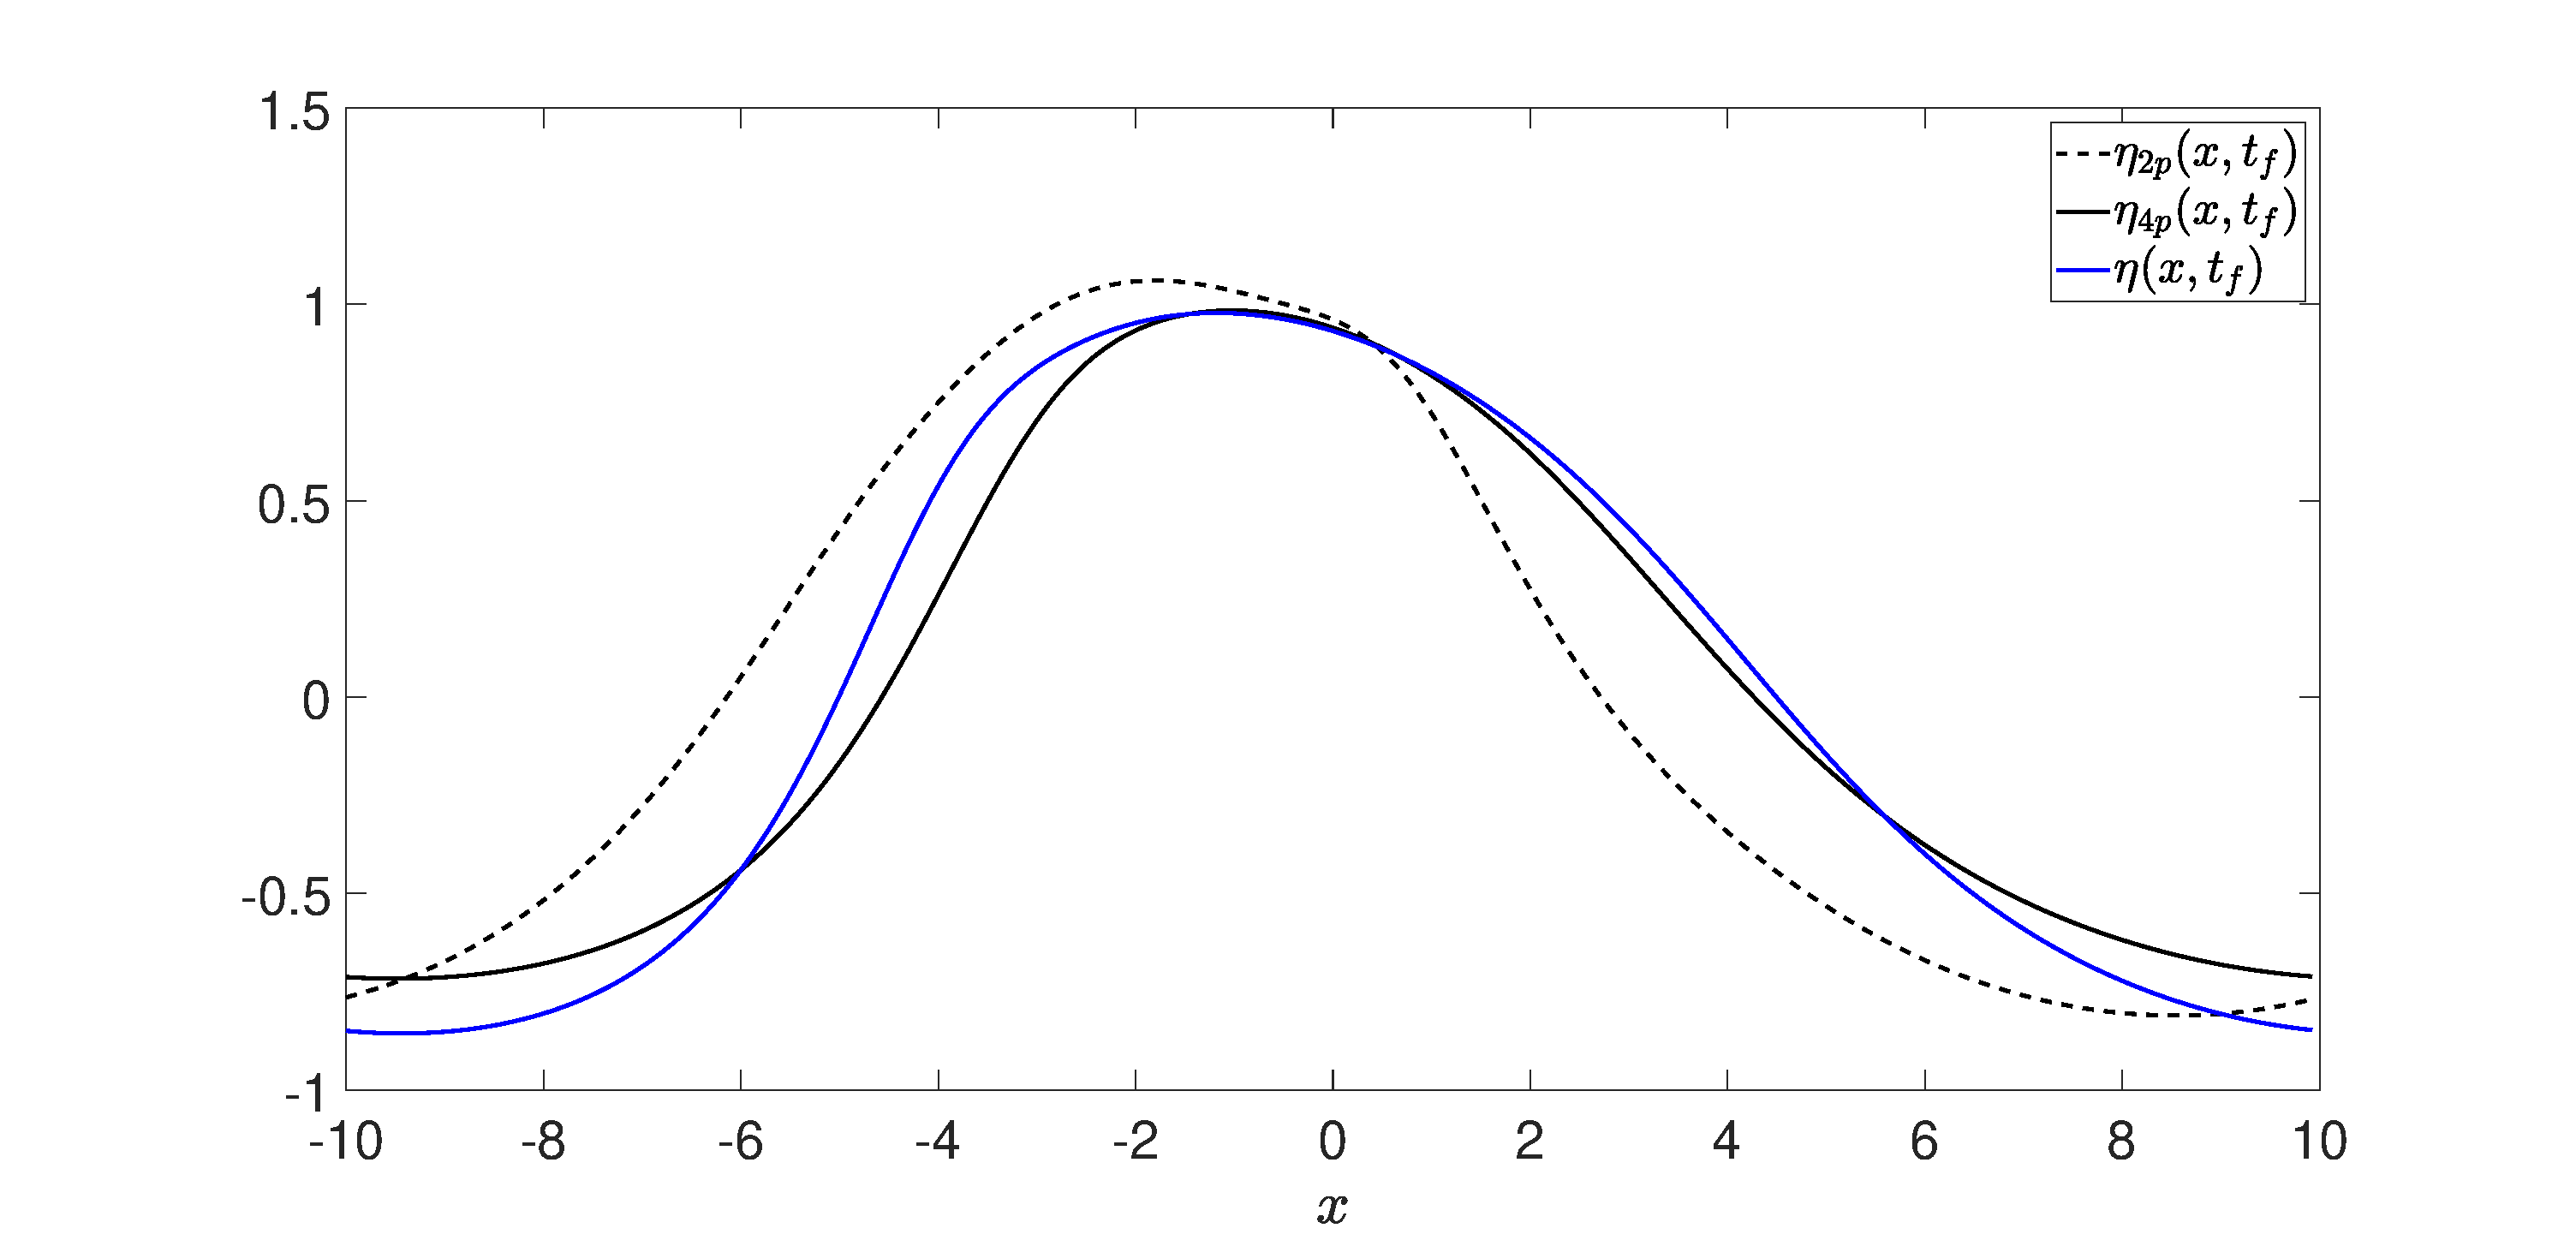
\includegraphics[width=.8\textwidth]{./Images/pwise_sig_pt1_srate_pt5_Nens_200_Np_4_tf_20_M_1}\\
		(a)\\
		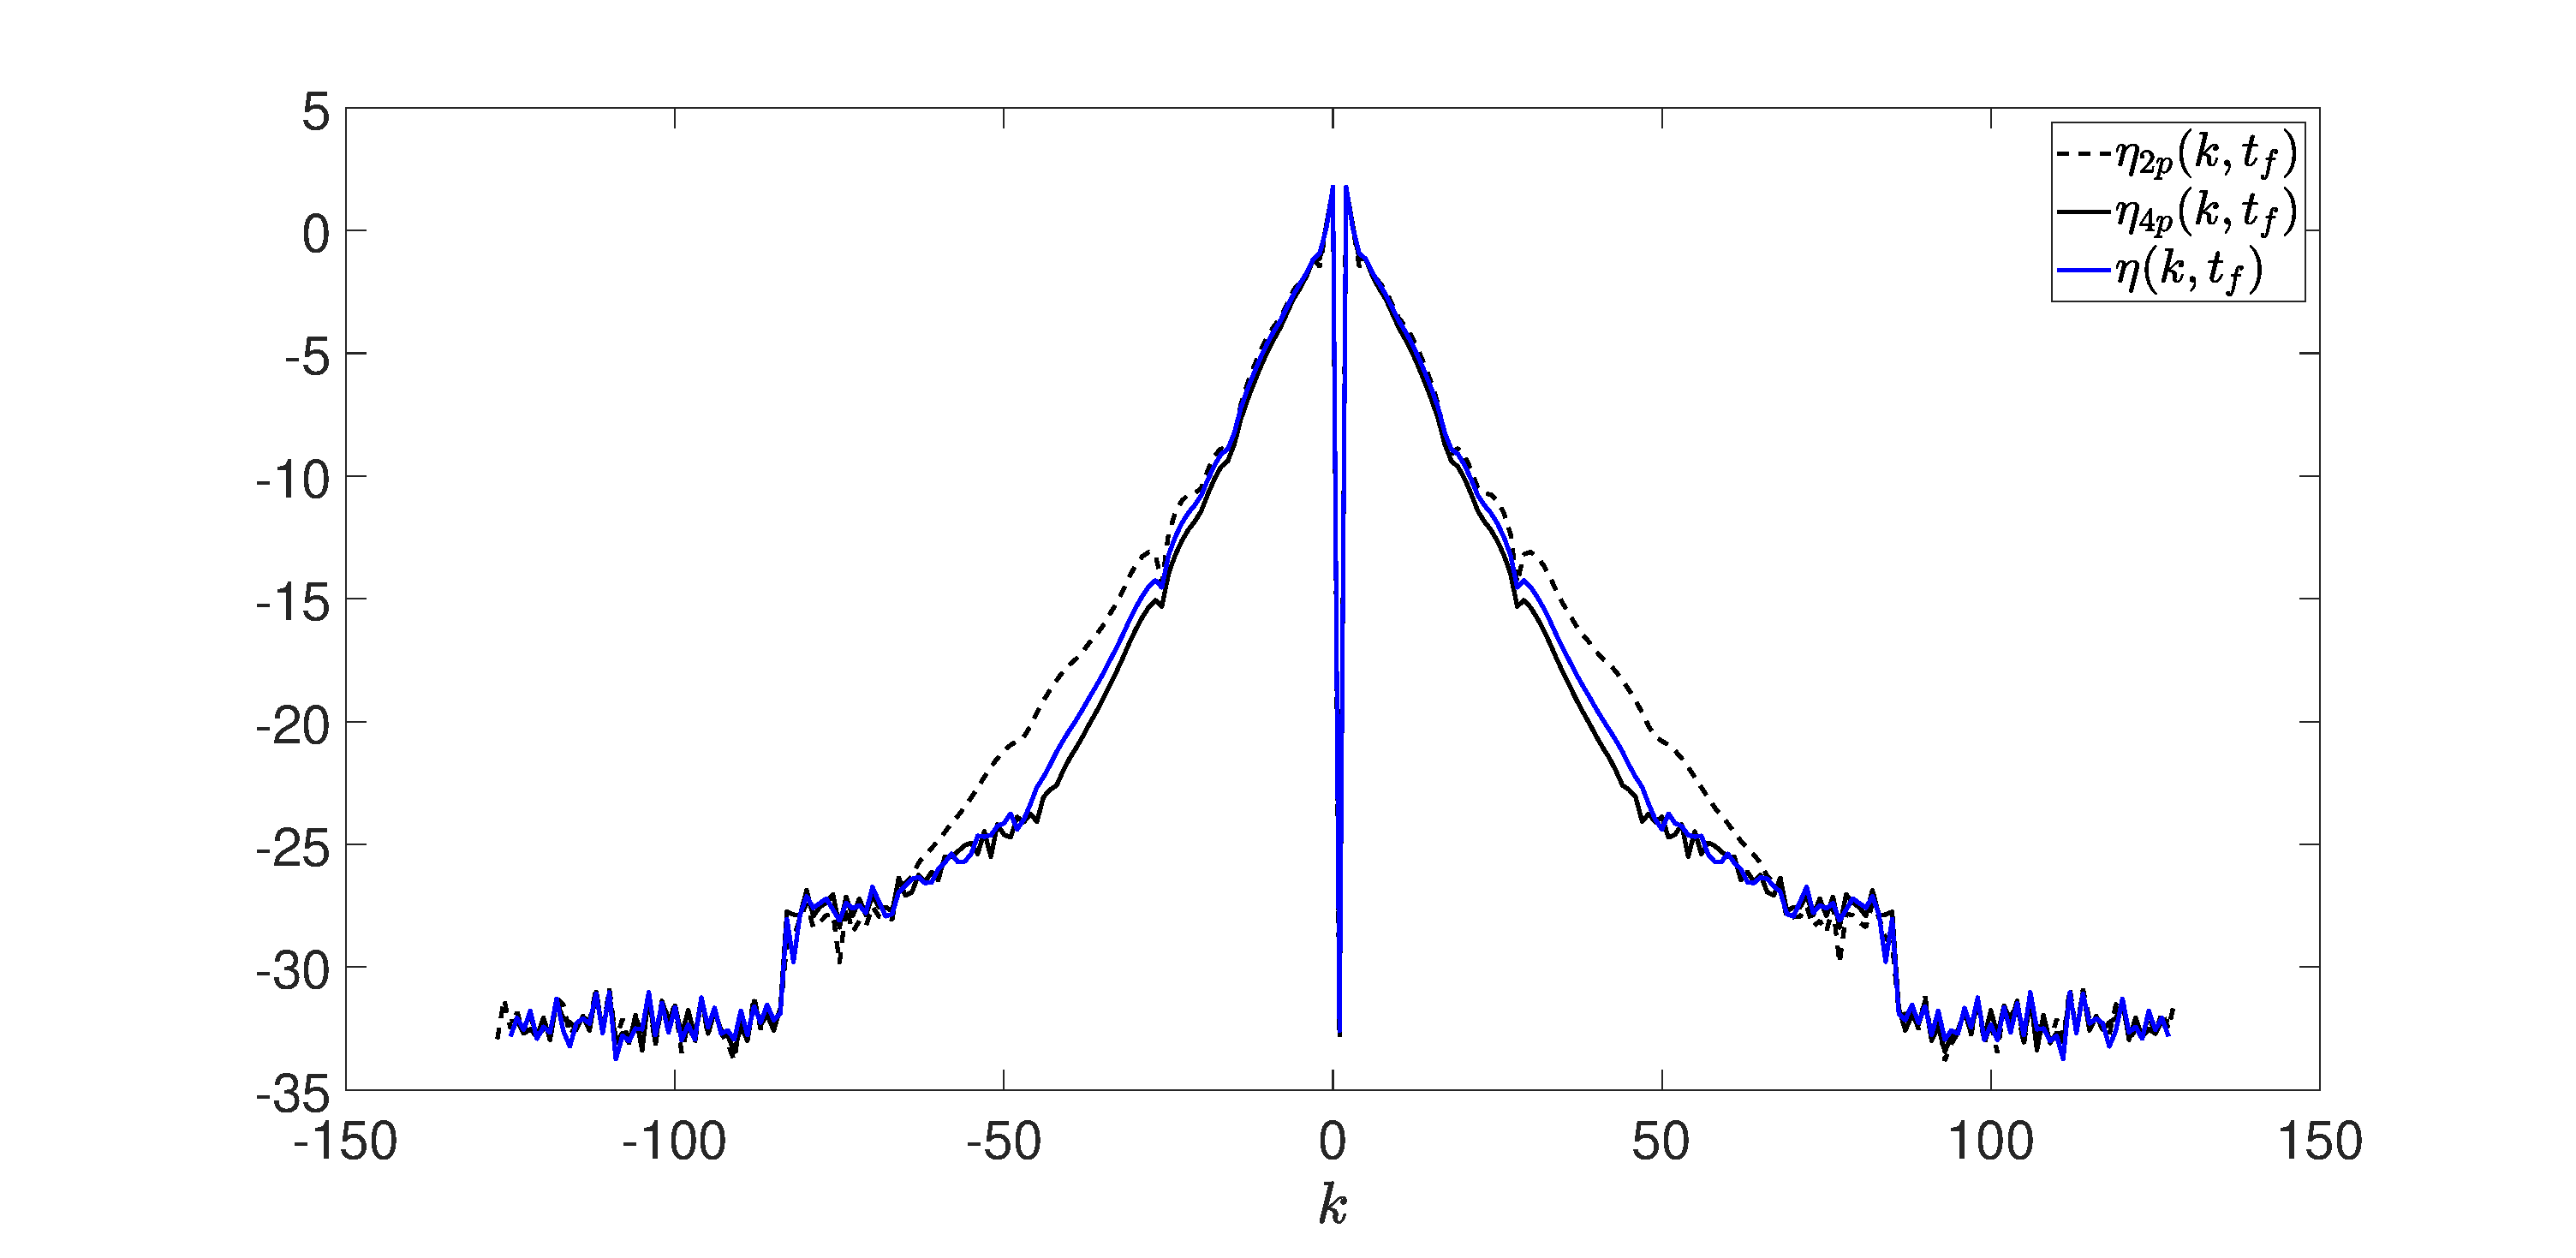
\includegraphics[width=.8\textwidth]{./Images/pspec_sig_pt1_srate_pt5_Nens_200_Np_4_tf_20_M_1}\\
		(b)\\
		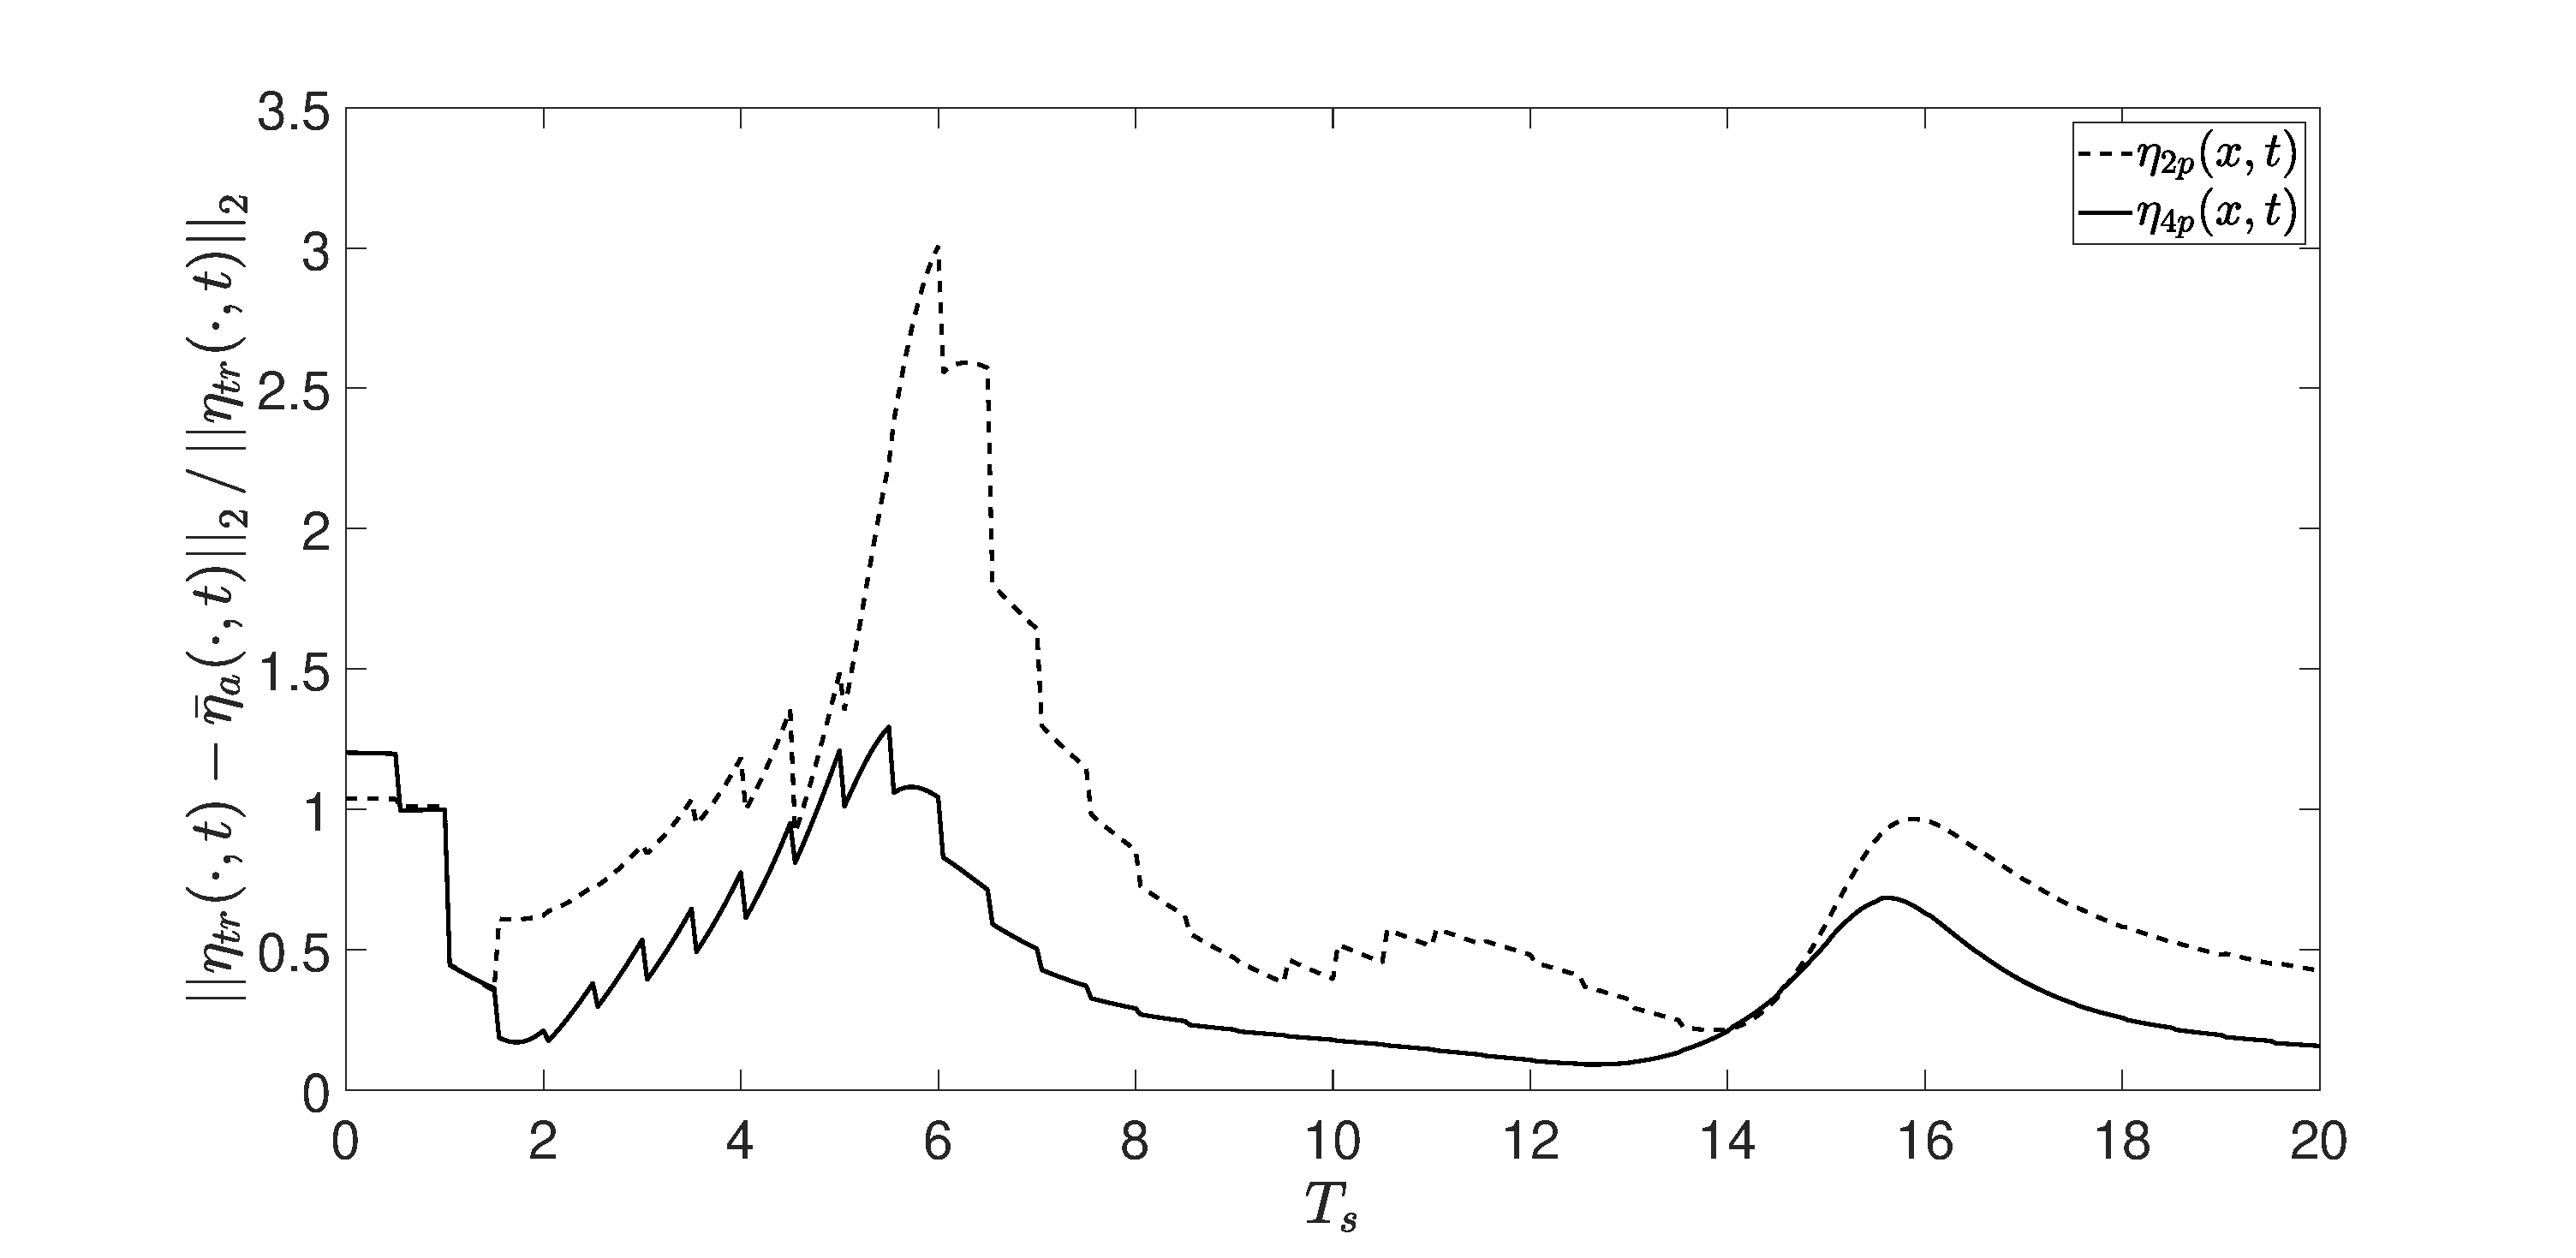
\includegraphics[width=.8\textwidth]{./Images/error_sig_pt1_srate_pt5_Nens_200_Np_4_tf_20_M_1}\\
		(c)	
	\end{tabular}	
	\caption{The pointwise-approximations (a) and power-spectrum approximations (b) at $t_{f}=20$, and error (c) measuring at two (- -) and four points (--) using $M=1$ terms in the DNO.  The data-assimalation rate is $\delta t_{s}=.5$, so that the model is predicting behavior in between assimation events.}
	\label{fig:dno_1}
\end{figure}

\begin{figure}[!h]
	\begin{tabular}{c}
		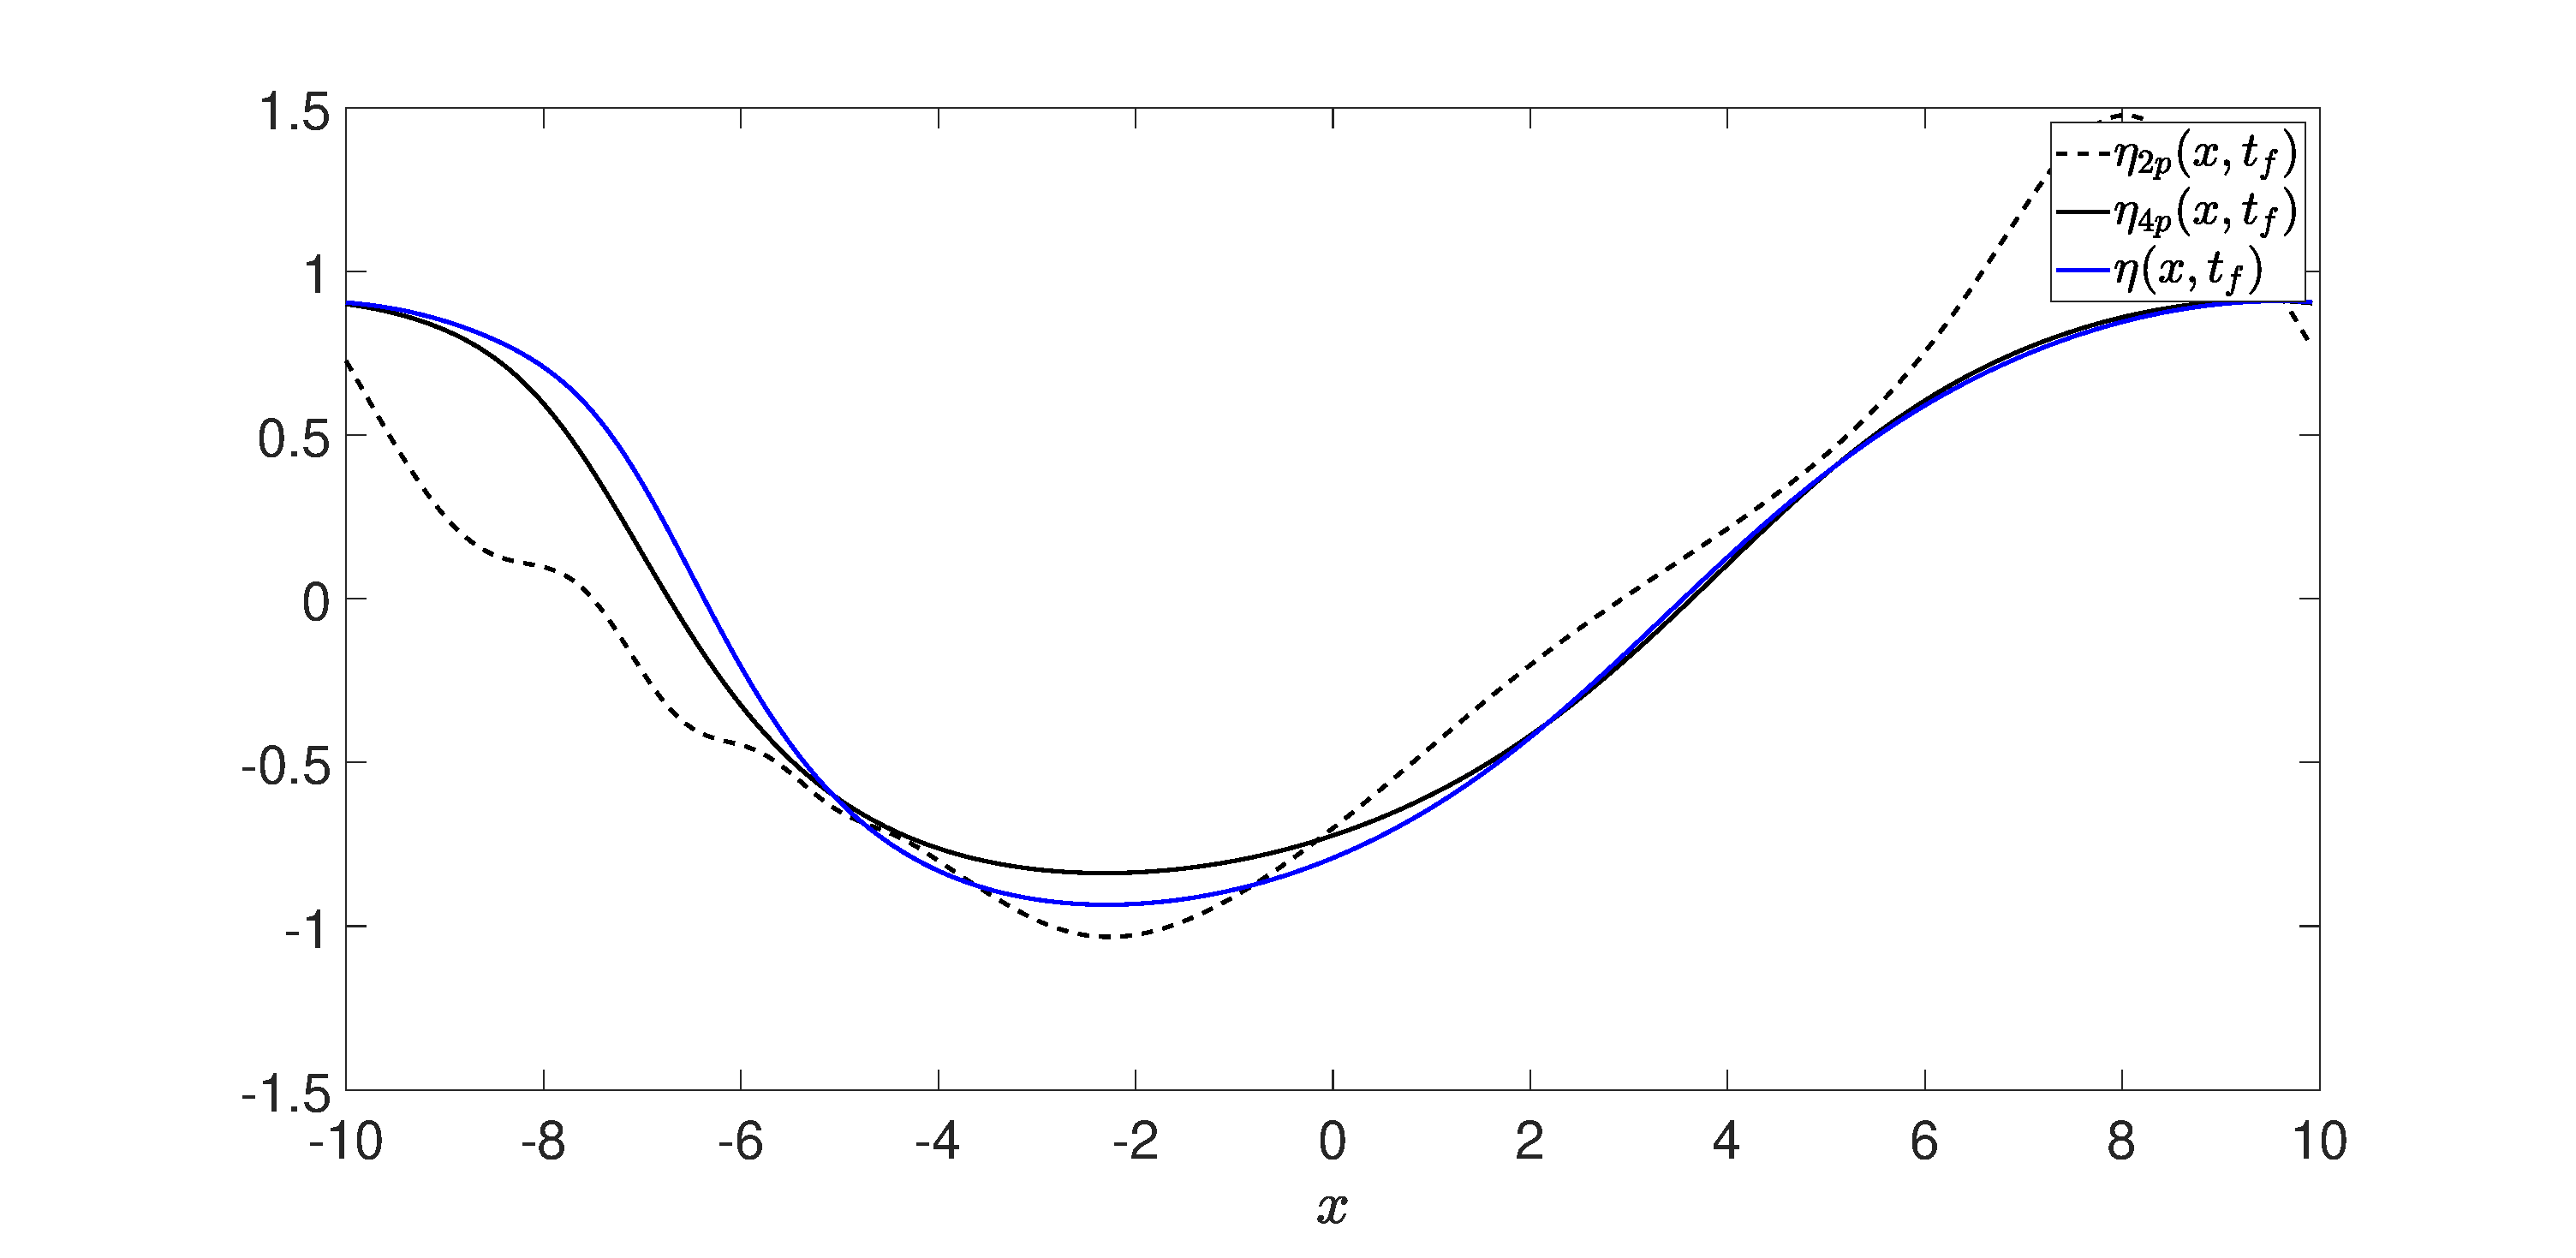
\includegraphics[width=.8\textwidth]{./Images/pwise_sig_pt1_srate_pt5_Nens_200_Np_4_tf_20_M_14}\\
		(a)\\
		\includegraphics[width=.8\textwidth]{./Images/pspec_sig_pt1_srate_pt5_Nens_200_Np_4_tf_20_M_14}\\
		(b)\\
		\includegraphics[width=.8\textwidth]{./Images/error_sig_pt1_srate_pt5_Nens_200_Np_4_tf_20_M_14}\\
		(c)	
	\end{tabular}	
	\caption{The pointwise-approximations (a) and power-spectrum approximations (b) at $t_{f}=20$, and error (c) measuring at two (- -) and four points (--) using $M=14$ terms in the DNO.  The data-assimalation rate is $\delta t_{s}=.5$, so that the model is predicting behavior in between assimation events.}
	\label{fig:dno_14}
\end{figure}

However, what is perhaps surprising is the degree to which a relatively modest amount of nonlinearity enhances the overall accuracy of our assimilation/prediction approach; compare the two-point assimilation error in Figure \ref{fig:dno_1} (c) to that in Figures \ref{fig:dno_0} (c) and \ref{fig:dno_14} (c).  Thus it seems appropriate amounts of nonlinearity can potentially enhance otherwise unusuable sparse measurement schemes.  

Of concern though is the common increase in error around $t=15$ in each of the plots of $\mathcal{E}(t)$.  To what extent this can be mitigated so that a more uniformly reliable assimilation/approximation scheme can be developed is question of ongoing research.  
%%%%%%%%%%%%%%%%%%%%%%%%%%%%%%%%%%%%%%%%%%%%%%%%%%%%%%%%%%%%%%%%%%%%%%%%%%%%%%%%%%%